\documentclass[twocolumn]{revtex4}
\usepackage{graphics,graphicx,epsfig,ulem,amsmath,multirow,gensymb,commath,textcomp,natbib,blindtext}
\newcommand{\squeezeup}{\vspace{-2.5mm}}

\begin{document}

\textheight=26.385cm
%Change textheight as the last resort...

\title{Investigating and understanding diffraction patterns using Fourier analysis with variations of the $\boldsymbol{4f}$ Optical System}
 
\author{Jacky Cao, Fourier Optics, Friday, Lab Partner: Thomas Spriggs \\ Dates of experiment: 10/02/2017 to 17/03/2017, Date of report: 19/03/2017}

\begin{abstract}              
Through the study of Fourier transforms it has been possible to understand diffraction gratings and their patterns. Using a $4f$ optical system illuminated by a coherent laser, diffraction patterns in different viewing planes can be observed using a CCD camera. Quantitative data can be collected by comparing the intensity profiles of the patterns with a theoretical model, our reduced $\chi^2$ values ranged from 36.8 (single slit) to $3.63\times10^5$ (five slits), indicating that the fittings were not suitable \cite{hughesandhayes}. Improvements to the experimental procedure are required to improve the quality of data. 
\end{abstract}

\maketitle

\section{Introduction} 
\vspace{-2ex} 

In the field of optics, a diffraction pattern can be produced when a coherent beam of radiation falls onto a partially opaque object \cite{mathmethods}. The pattern can then be viewed at a ``far-field'' distance - a distance that is great. This length is larger than the initial size of the object, allowing for the spreading of light due to diffraction to dominate in the  plane of observation \cite{of2f}. 

The applications of diffraction patterns includes the study of crystalline structures. Through X-ray and electron diffraction it is possible to obtain accurate information about the identity of phases present, atomic ordering, and for recognising different metallurgical constituents within a specimen. This allows for potential applications within areas such as the pharmaceutical industry, where early analysis of different mixtures and compounds can be cost and time saving. \cite{elecdiffraction, xraypharma}

Another application could potentially involve using the diffraction pattern within an illumination system so that X-ray phase contrast microscopy and interferometry can be performed \cite{singleslit}. This could be used to enhance the visibility of fine scale structures, which would be especially useful in biology as quantitative data can be obtained about a sample from just phase-contrast images \cite{xrayphase}.

With these varying applications we find that in order to fully understand diffraction patterns and how they are formed, we must look at the mathematics behind them. 

The main mathematical tool that we must use in building our understanding is Fourier analysis, more specifically, Fourier transforms. A Fourier transform is a way of representing a function in terms of a superposition of sinusoidal functions, with the explicit conditions of the function being defined over an infinite interval and having no particular periodicity \cite{mathmethods}.

\textit{The following theory/mathematics has been adapted from Optics f2f} \cite{of2f}.

The Fourier transform $F(u)$ of a single function $f(x)$ can be stated as,
\begin{equation}
F(u) = \mathcal{F}[f(x)](u) = \int_{-\infty}^\infty f(x) e^{-i2\pi ux}dx,
\label{fourierdefinition}
\end{equation}

where $(u)$ is the dependent Fourier variable. This expression tells us the spectrum of frequencies required to form the function $f(x)$.

We can also algebraically manipulate the initial function before Fourier transforming it. In Table \ref{fourierproperties} we find the group of functions known as the Fourier transform properties.
\begin{table}[h!]
\centering
\begin{tabular}{c@{\hskip 20pt}c@{\hskip 20pt}c@{\hskip 20pt}c} 
 \hline
 \textbf{Property} & \textbf{$\boldsymbol{f}$} & \textbf{$\boldsymbol{F}$} \\ [0.5ex] 
 Linearity				& $g(x)+h(x)$ & $G(u) + H(u)$ \\
 Translation 			& $f(x-a)$ 	& $F(u)e^{-i2\pi ua}$ \\ 
 Scaling 				& $f({x/a})$ & $aF(ua)$ \\
 Convolution			& $(g*h)(x)$ & $GH$ \\
 Inverse Convolution		& $gh$ & $ (G*H)(u)$ \\
 \hline
\end{tabular}
\caption{The Fourier transform properties - functions $\boldsymbol{f}$ and their output $\textbf{$\boldsymbol{F}$}$ when they have been Fourier transformed using equation \ref{fourierdefinition}.}
\label{fourierproperties}
\end{table}

The convolution property can be better understood as follows: if we convolve two functions of $x$, $g(x)$ and $h(x)$, then that can be defined as,
\begin{equation}
(g*h)(x) = \int_{-\infty}^\infty g(x')h(x-x') dx'.
\end{equation}

Stated in words, a convolution is \textit{sliding one function through the other and summing the area which overlaps}. This can be especially useful if we are translating a function and making multiple copies of it.

In the application of optics, the Fourier variable that we have stated as $u$ is called the spatial frequency. It is defined as the \textsl{number of waves per unit length}, and is the real space analogue of frequency. It's mathematical form for the far-field case can be written as a mapping between the Fourier variable and real space position,
\begin{equation}
u=\frac{x}{\lambda z},
\end{equation}

where $x$ is the position in real space, $\lambda$ is the wavelength of radiation being used to illuminate the object, and $z$ is the distance ``downstream'' from the object.

When considering diffraction gratings, we can describe the physical makeup of one using a mathematical function. This function could then be manipulated using the different Fourier transform properties as found in Table \ref{fourierproperties}. The result of which is an expression which can reproduce and describe the diffraction pattern that is observed. 

When working with optics we must make the distinction between \textit{real} and \textit{Fourier} space. The former indicating the plane in which a diffraction grating would sit, and the latter representing the plane when the diffraction grating (or radiation) has been Fourier transformed. 

There are some basic shapes that can be used as the object which is being illuminated on by radiation: a rectangular slit, and a circular aperture. However, to consider these cases we must move into 2 dimensions and consider a 2D Fourier transform. 

A 2D Fourier transform has the form of a double integral, equation \ref{fourierdefinition} thus becomes,
\begin{equation}
F(u,v) = \int_{-\infty}^{\infty} \int_{-\infty}^{\infty}f(x,y)e^{-i2\pi(ux+vy)}dxdy,
\end{equation}
where $u$ and $v$ are the spatial frequencies corresponding to the $x$ and $y$ directions respectively - an extra set of terms must now be considered within our calculations.

In Table \ref{fshapes} we find the functional form of the rectangular and circular shapes and their output when they are Fourier transformed. Their derivations can be found on pp. 63-64 of \textit{Optics f2f} \cite{of2f}. 
\begin{table}[h!]
\centering
\begin{tabular}{c@{\hskip 20pt}c@{\hskip 20pt}c@{\hskip 10pt}c} 
 \hline
 \textbf{Shape} 	& \textbf{$\boldsymbol{f}$} 		& \textbf{$\boldsymbol{F}$} \\ [1ex] 
 Rectangle 	& $\text{rect}(x/a)$ 				& $a\: \text{sinc}(\pi ua)$ \\ 
 Circle 		& $\text{circ}(\rho/D)$ 			& $(\pi D^2/4)\: \text{jinc}(\pi \varpi D)$ \\
 \hline
\end{tabular}
\caption{Function of each shape and it's Fourier transform. Where $a$ is the width of a rectangular pulse, $\rho=\sqrt{x^2+y^2}$ is the radial distance, $\varpi=\sqrt{u^2+v^2}$ is the Fourier equivalent of this, and $D$ is the diameter of the circle.}
\label{fshapes}
\end{table}
\setlength{\belowcaptionskip}{-10pt}

With the one dimensional \textit{rect} function, the Fourier function is a \textit{sinc}, this can be defined in the more familiar terms of $\text{sinc}(\pi ua)=\sin (\pi ua)/(\pi ua)$. Similarly, the result for the \textit{circ} is a \textit{jinc} function, which is essentially a Bessel function of the first order. Rewritten, it is: $\text{jinc}(\pi \varpi D)=J_1 (\pi \varpi D)/(\pi \varpi D)$.

To repeat one of these functions one can use a \textit{comb} function - a sum of regularly spaced $\delta$-functions. In the context of optics, the real space $\delta$-function contains all spatial frequencies with an equal amplitude. We can Fourier transform the $\delta$-function so that $\mathcal{F}[\delta(x)](u)=1$.

Defining the comb function as an algebraic summation, it's expression is thus given as,
\begin{equation}
\text{comb}_N \Big(\frac{x}{d}\Big) = \sum_{n=-(N-1)/2}^{(N-1)/2} \delta(x-nd),
\end{equation}

where the argument $x$ has been scaled by the value of $d$ in comb, and $N$ is the number of $\delta$-functions.

If we were to Fourier transform this finite comb, then the outcome is a discrete sum of phasors, 
\begin{multline}
\mathcal{F}\Big[\text{comb}_N\Big(\frac{x}{d}\Big)\Big](u)=e^{-i(N-1)\pi ud} + e^{-i(N-1)\pi ud}e^{i2\pi ud}\\+...+e^{i(N-1)\pi ud}.
\end{multline}

This is useful to us in optics as diffraction gratings can expand from being a single aperture to many apertures e.g. a single slit versus a coarse grating of many slits.

We can relate the maths to experiment through shining coherent radiation onto a diffraction grating and then observing the diffraction pattern at some distance. 

What is observed can be quantified in terms of the \textit{intensity}, this is found by taking the absolute value of the Fourier transform, squaring it, and applying a scaling factor $I_0/(\lambda^2z^2)$ - where $I_0$ is a number, $\lambda$ is the wavelength of radiation, and $z$ is the distance `downstream'.

Using an optical system which composes of a laser and two identical lenses, the radiation of the laser passing through a diffraction grating can be focused to distances equal to multiples of the focal length of the lenses. The resulting pattern can then be observed on a screen or with a CCD. The setup in mind is called the $4f$ optical system - where each component is a focal length, $f$, apart.

The laser and the lenses have their own mathematical descriptions attributed with them.

The profile of the laser beam is of a \textit{gaussian} shape, the mathematical definition and Fourier transform of it can be found in \textit{Optics f2f}. The lenses act as a magnifier, this results in the diffraction pattern shifting from being at a far-field distance $z$, to the focal length distance $f$ of the lens.

Using variations of the $4f$ system we can explore and study different diffraction patterns and relate them back to their mathematics.

\vspace{-3ex}
\section{Method} 
\vspace{-2ex}
To create and observe diffraction patterns we needed to set-up the $4f$ system. Figure \ref{m-fig1} shows this experimental setup.
\begin{figure}[!h]
\begin{center}
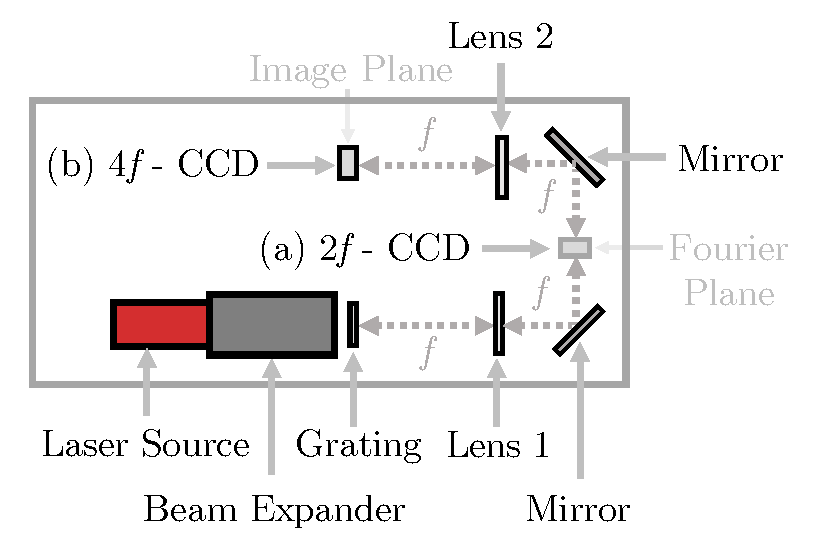
\includegraphics[width=6.5cm]{method/fig1-1}
\caption[]{A plan view schematic of the experimental set-up used to collect data. $f$ are the focal lengths of lenses 1 and 2. Each component was attached to an optical breadboard. (a) $2f$ optical system used in studying the Fourier plane. (b) $4f$ optical system used in studying the image plane.}
\label{m-fig1}
\end{center}
\end{figure}

A coherent laser source of wavelength $\sim635$ nm was used as our source of radiation. A $\times10$ beam expander was placed directly after this to allow the beam width to be adjusted during experimentation, this was done in an attempt to focus the majority of the light onto the area of the diffraction grating.

To place the lenses at the correct $f$ distances their focal lengths had to be measured. This was done by placing each lens at the beam expander, then moving a screen closer and further away from the source until the brightest and sharpest spot could be observed. At that distance was thus the focal length, measured with a metre ruler we found that for both lens 1 and 2, their focal lengths were $48\pm1$ cm.

Due to the constraint with the length of the breadboard, two mirrors were used to reflect the light into a CCD camera so that the set-up would take up less space.

The camera was moved at various stages of experimentation, from being in the Fourier plane at a distance of $2f$, to a distance of $4f$ when we wanted observations to be made within the image plane.

Our CCD was controlled using the provided manufacturer's software, images were saved and then later analysed using modules created in Python and in MATLAB. 

The programs would convert the image from RGB colour into grayscale, calculate intensity profiles for the $x$ and $y$ directions of the image, and then attempt a model fitting with a chosen model.

The grayscale images were obtained by converting the three RGB values from a pixel into a singular value defined by the CIE 1931 Linear Luminance,
\begin{equation}
Y_{\text{linear}}=0.2126R+0.7152G+0.0722B,
\end{equation}

where $R,G,B$ are the respective \textit{red}, \textit{green}, and \textit{blue} values from the pixel \cite{rgbtogray}. This greyscale intensity has no particular units, but a fixed range between 0 (total black) to 255 (total white). The camera had a bit-depth of 8, thus it can distinguish between 256 intensity levels.

The intensity profiles were created by locating the rows (and columns) within the images that contained the greatest amount of pixels with the maximum intensity value of 255, these were then averaged together. 

A graph could then be plotted, and subsequently a $\chi^2$ value could be calculated when a theoretical model was compared to the intensity graphs.

These models were derived from the mathematics of Fourier transforms, as found in \textit{Optics f2f} \cite{of2f}.

Throughout our research we varied the gratings that were used, they were placed within a holder just after the beam expander and the pattern that they created was observed at different distances. 

Adjustments had to be made so that the pattern observed was as clear as possible. A recurring problem was the over-saturation of the image of the diffraction pattern. This was corrected for by using a neutral density filter and adjusting the exposure time and the gain of the CCD within the software.

To measure small scale distances of features on the diffraction grating, a travelling microscope with a Vernier scale was used.

\vspace{-3ex}
\section{Results}
\vspace{-2ex}
Figure \ref{horizontal_profiles} show multiple plots of the horizontal intensity against the distance along the $x$ direction in pixels for different diffraction patterns in the Fourier plane. 
\begin{figure}[!h]
\begin{center}
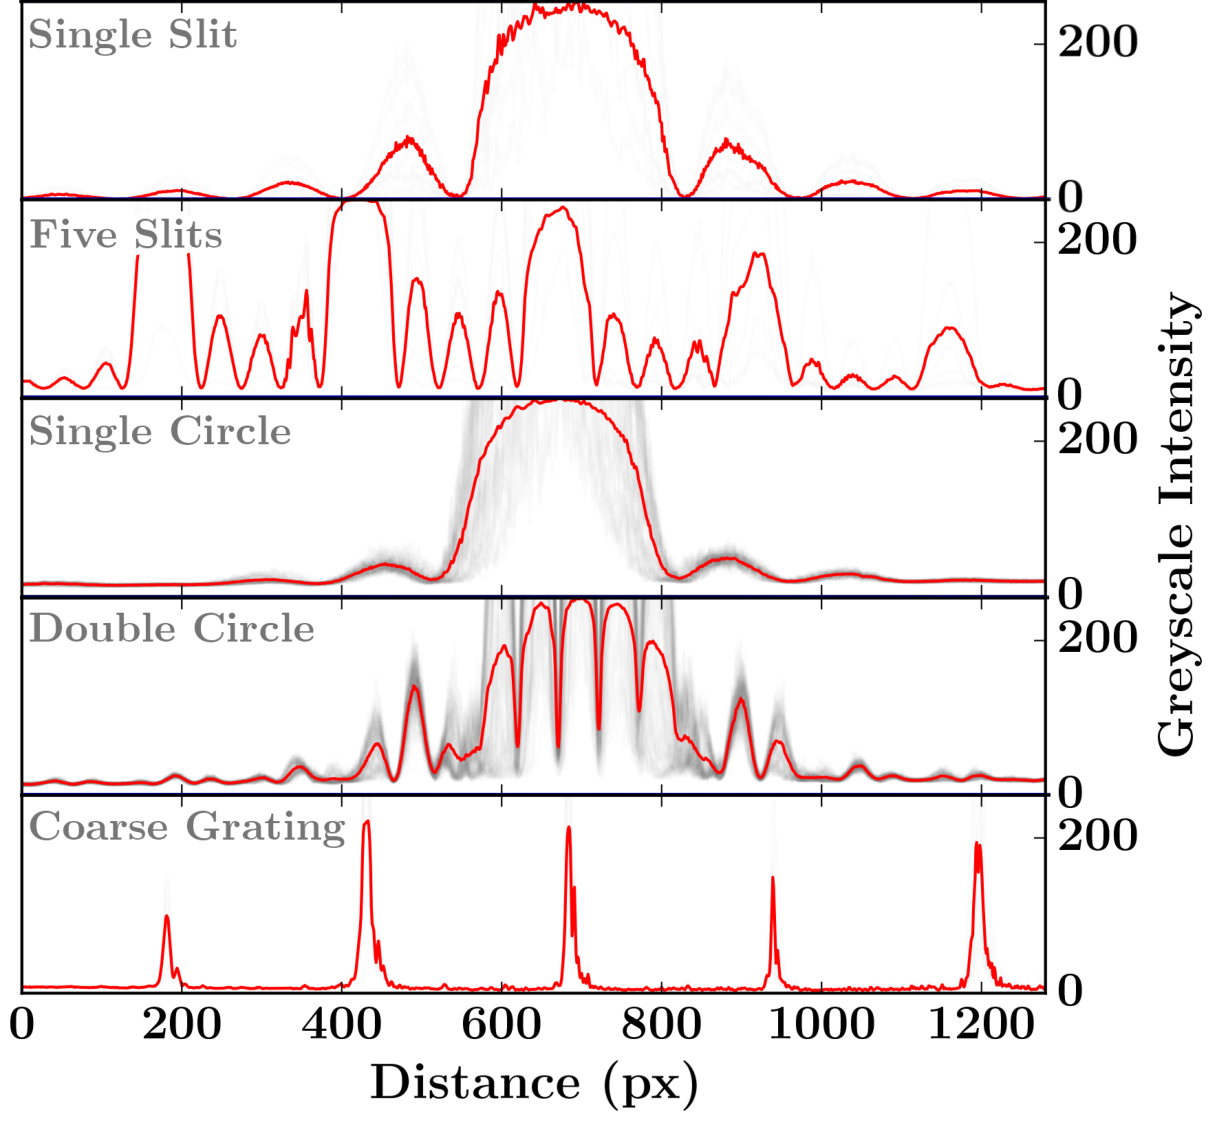
\includegraphics[width=7cm]{results/horizontal_intensity_profiles3}
\caption[]{Horizontal intensity profiles of diffraction patterns within the Fourier plane. The error bars are too small to be seen.}
\label{horizontal_profiles}
\end{center}
\end{figure}
\begin{figure}[!h]
\begin{center}
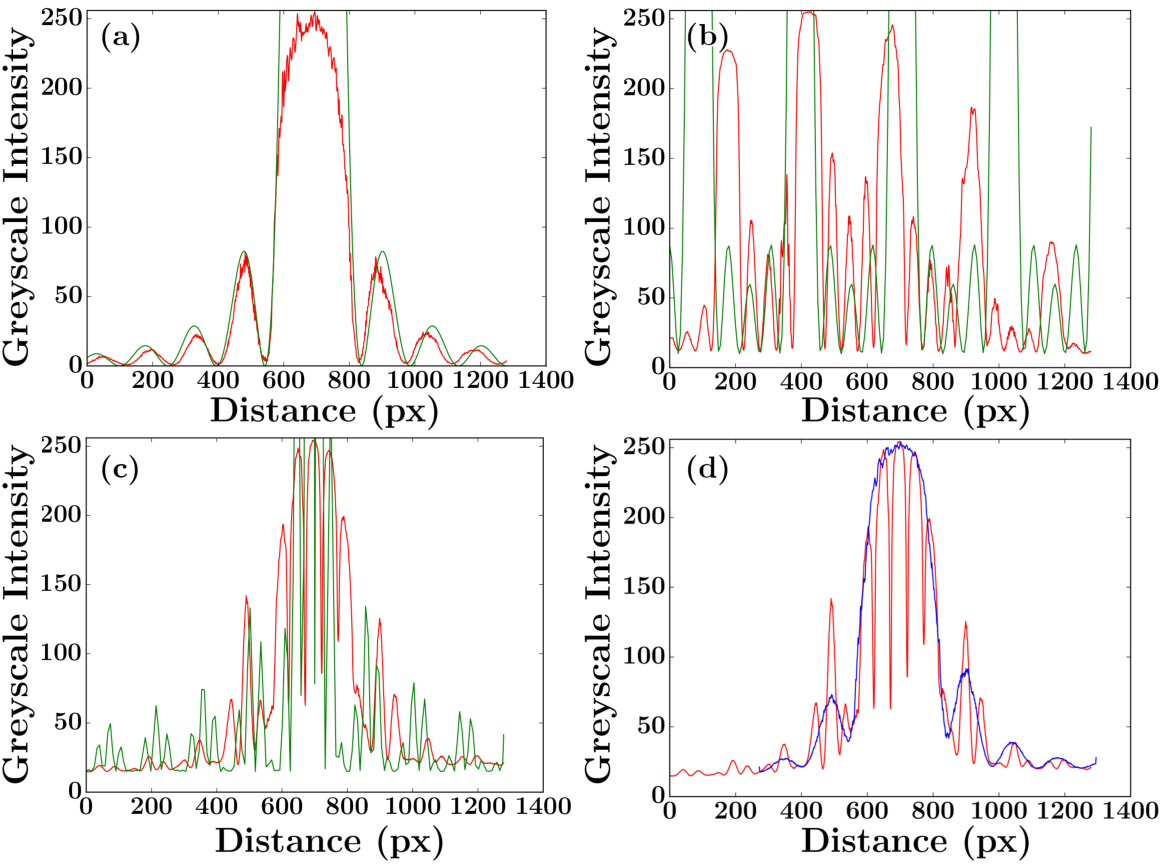
\includegraphics[width=9cm]{results/data_and_models2}
\caption[]{Theoretical model (green), horizontal intensity data (red), and vertical intensity data (blue) - data taken in the Fourier plane. The uncertainties for the horizontal and vertical intensities are too small to be seen. (a) Single slit with model. (b) Five slits with model. (c) Double circles with model. (d) Envelope nature of double circle slit.}
\label{datamodels}
\end{center}
\end{figure}

Figures \ref{datamodels}(a), \ref{datamodels}(b), and \ref{datamodels}(c) show the horizontal intensity data for the single slit, five slits, and double circle slit plotted with a theoretical model. The reduced $\chi^2$ values have been calculated and can be found in Table \ref{theoretical_model_applying}.

The horizontal and vertical intensity graphs for the double circular slit have been superimposed and can be found in Figure \ref{datamodels}(d).

Table \ref{realtofourier} shows the slit widths of three different coarse gratings as measured in real space, and calculated from Fourier space.

Figure \ref{collage} shows intensity maps of diffraction patterns took as part of extensions to our research.

\begin{table}[h!]
\centering
\begin{tabular}{c@{\hskip 20pt}c@{\hskip 20pt}c@{\hskip 20pt}c} 
 \hline
 \textbf{Grating} & $\boldsymbol{\chi_\nu^2}$ \\ [0.5ex] 
 Single Slit &$36.8$ \\ 
 Five Slits & $3.63\times10^{5}$ \\
 Double Circle & $6.55\times10^{4}$ \\
 \hline
\end{tabular}
\caption{A theoretical model was applied to the single slit, five slits, and double circle diffraction gratings. Their respective reduced $\chi^2$ statistic have been calculated. \\}
\label{theoretical_model_applying}
\end{table}
\begin{table}[h!]
\centering
\begin{tabular}{c@{\hskip 15pt}c@{\hskip 15pt}c@{\hskip 10pt}c} 
 \hline
 \textbf{Grating} & \textbf{Real Space [mm]} & \textbf{Fourier Space [mm]} \\ [0.5ex] 
 $1$ &$0.20\pm0.05$ & $0.11\pm0.03$ \\ 
 $2$ & $0.12\pm0.05$ & $0.11\pm0.01$ \\
 $3$ & $0.08\pm0.05$ & $0.05\pm0.01$ \\
 \hline
\end{tabular}
\caption{For each coarse diffraction grating, the diffraction grating slit width is shown as measured in real space, and as calculated in Fourier space. \\}
\label{realtofourier}
\end{table}
\begin{figure}[!h]
\begin{center}
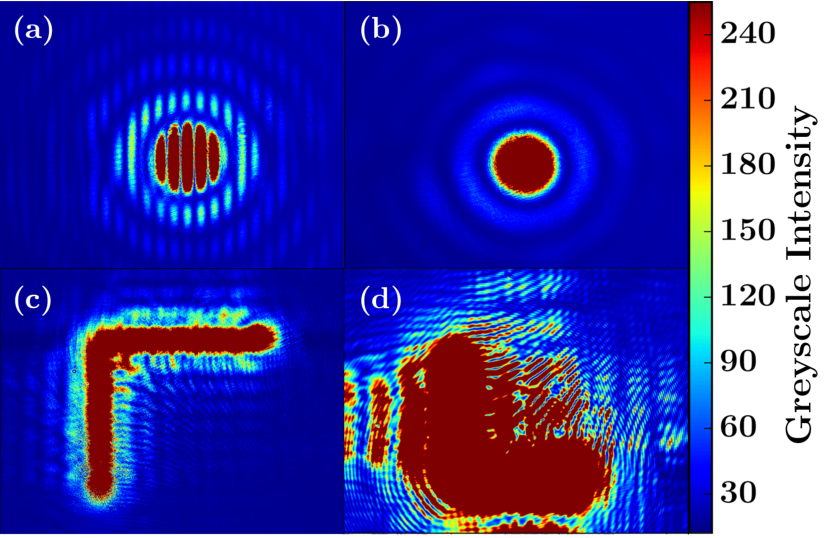
\includegraphics[width=8cm]{results/collage3}
\caption[]{Intensity maps of four different diffraction patterns taken from different planes: (a) double circle grating in Fourier plane, (b) single circle grating in Fourier plane, (c) L grating in image plane, (d) L grating in `$3f$' plane.}
\label{collage}
\end{center}
\end{figure}

\vspace{-3ex}
\section{Discussion}
\vspace{-2ex}
From just an initial inspection of Figure \ref{horizontal_profiles} we can discern the possible mathematics involved with the diffraction patterns.

We can see the application of the convolution theorem within the functions for the five slits and the double circle grating. They are respectively, a rect convolved with a comb$_5$, and a circ convolved with a comb$_2$. 

Looking at the calculated reduced $\chi^2$ values for these two gratings we see that they are not near unity at all, in fact they are orders of magnitude out. The basic requirement for the theoretical models to be a good fit to the data  is that they be close to the value of $1$ \cite{hughesandhayes}. For the single slit rect we see that the model used provides a closer fit than the others, but it is still not good.

While we do understand the functions of the gratings and conversely their Fourier transforms, there is much difficulty in implementing this within a program. The trouble mainly arises in attempting to scale and translate the model to fit the data - there is a large sensitivity in changing variable values, thus large $\chi^2_{\nu}$.

The images that we collected are not perfect, we can observe this with the intensity profile for the five slits. The principal maximas should all be the same height, as well as the first and last subsidiary maximas. This inevitably leads to a difficult fit with the model. We understood that this arose partially from saturation, and also from the laser beam not producing an even illumination, instead it was a non-uniform gaussian beam.

We selected to further understand the double circle slit. It's pattern of the convolved circ function retains it's original Airy disk profile but now also contains cos$^2$ interference fringes [see Figures \ref{collage}(a) and \ref{collage}(b)]. If the horizontal intensity of this is superimposed with a jinc$^2$-type intensity, then one can fit into the other in an envelope like nature [see Figure \ref{datamodels}(d)]. This is similar to the sinc$^2$ enveloping of Young's double slit experiment \cite{of2f}.

In developing our knowledge of real and Fourier space, we attempted to measure the slit width of a single slit of three different coarse gratings in real space and from Fourier space. The function of a coarse grating being a rect convoluted with comb$_N$, with $N$ being the number of slits - often a value larger than 10. Our results are shown in Table \ref{realtofourier}, we see that not all the measurements from real space agree with their calculated Fourier counterpart within their experimental error.

We suspect this could be due to how we defined the size of a pixel in Fourier space, our calculations for the first and third gratings were based off how we calculated what one pixel equals in Fourier space ($37\pm6$m) for the second grating. If this was incorrect, which we assume it was, then our other values are incorrect too.

After exploring patterns within the Fourier plane, we then moved into the image plane. In Figure \ref{collage}(c) the pattern is a rotated L shape, the original L grating was the `correct way up'. We can imagine the L grating as two perpendicular rects with one translated to the left. We find from the images that there has been a parity change from ($x,y$) to ($-x,-y$), this is not so obvious in the $x$ direction. This occurs when we take the Fourier transform of the field in the Fourier plane - it then becomes an inverse transform \cite{of2f}. 

A curious expansion to our research can be seen in Figure \ref{collage}(d). For this we moved the source and grating to be directly behind the first lens - a `$3f$' system. This pattern has features from both the Fourier and image plane. In the centre there is a clear \textit{L}, something as seen before in the image plane, and to the sides we can view what appears to be Fourier plane sinc$^2$ fringes. While we did not explore the mathematics for this, we could suggest that this pattern was formed by applying a convolution to the initial function as it has retained features from both planes.

Further experimentation would certainly be required to validate or disprove this.

Improvements could be made to our investigation to improve the quality of data taken. Considerations of noise is one - bias and readout noise, as well as dark current could be measured, and their effect could be removed from any images taken. A laser source which produces even illumination could also be used so that it provides more uniform data which is closer to the model, thus improving the fit.

Extensions to our research could involve creating higher $f$ systems - would the pattern in a $6f$ system be just another inverse Fourier transform of the field from the image plane, and what would this pattern look like?

\vspace{-5ex}
\section{Conclusions}
\vspace{-2ex}

In conclusion it has been possible to investigate and understand different diffraction gratings and their patterns through the use of Fourier analysis.

Through producing diffraction patterns within a $4f$ optical system we have been able to observe how the properties of Fourier transforms can change a function, for example convolution has been observed with the five slits and double circle slit.

However, our quantitative data shows that more work has to be made in improving the quality of data, such as reducing saturation. This then would improve the fitting of models and enable us to make calculations between two different spaces more easily.

\begin{thebibliography}{5}
\bibitem{mathmethods}
	K. F. Riley, M. P. Hobson, and S. J. Bence.
	\textit{Mathematical Methods for Physics and Engineering}.
	Cambridge University Press, Cambridge, UK, 2010.
	
\bibitem{of2f}
	C. S. Adams and I. G. Hughes.
	\textit{Optics f2f, from Fourier to Fresnel}.
	Clarendon Press, Oxford, UK, 2017.

\bibitem{elecdiffraction}
	K. W. Andrews, D. J. Dyson, and S. R. Keown.
	\textit{Interpretation of Electron Diffraction Patterns}.
	Hilger \& Watts Ltd, London, UK, 1967.
	
\bibitem{xraypharma}
	J. P. Smit, R. B. McClurg.	
	\textit{X-ray Powder Diffraction Pattern Indexing for Pharmaceutical Applications}.
	Pharmaceutical Technology, January 2013, Vol. 37, No. 1.
	
\bibitem{singleslit}
	A. R. Lang, et al.
	\textit{Single-slit diffraction patterns of sub-nanometre-wavelength synchrotron radiation}.
	Journal of Physics D: Applied Physics, 1987, Vol. 20, No. 4, pp. 541-544.
	
\bibitem{xrayphase}
	S. C. Mayo, et al.
	\textit{X-ray phase-contrast microscopy and microtomography}.
	Optical Express, 2003, Vol. 11, No. 19, pp. 2289-2302.
	
\bibitem{rgbtogray}
	M. Stokes, et al.
	\textit{A Standard Default Color Space for the Internet}.
	November 1996, available at: https://www.w3.org/Graphics/Color/sRGB, accessed: 11th February 2017. 
	
\bibitem{hughesandhayes} 
	I. G. Hughes and T. P. A. Hase.
	\textit{Measurements and their Uncertainties}. 
	Oxford University Press, Oxford, UK, 2010.
	
\end{thebibliography}
\clearpage

\vfill
\twocolumngrid
\vspace{-3ex}
\section*{Appendix}
\vspace{-2ex}

In applying the theoretical models to our intensity data we had to measure features from the diffraction gratings using a travelling microscope with a Vernier scale. 

The slit width of the single slit grating, the width of a single slit from the five slit grating, and the diameters of the circles plus the distance between them for the double circle grating each have an individual uncertainty of $0.005$cm.

The following calculations were derived from \textit{Measurements and their Uncertainties} [I. G. Hughes and T. P. A. Hase, \textit{Measurements and their Uncertainties}, Oxford University Press, Oxford, United Kingdom, 2010].

The reduced $\chi^2$ statistics for the single slit, five slit, and double circle slit were calculated using this equation,
\begin{equation}
\chi^2_\nu = \frac{\chi^2}{\nu},
\end{equation}

where $\chi^2$ is the calculated chi-squared value, and $\nu$ the number of degrees of freedom. For each of the used gratings $\nu$ was chosen to be 1280 - this equates to the number of pixels in the image, in the horizontal direction.

To calculate $\chi^2$ the following formula was used,
\begin{equation}
\chi^2 = \sum_i \frac{(y_i -y(x_i))^2}{\alpha_i^2},
\end{equation}

where $y_i$ represents the theoretical model, $y(x_i)$ is the measured intensity data, and $\alpha_i$ is the uncertainty on that intensity.

As the data was found by averaging multiple rows (and columns) together, the uncertainty $\alpha_i$ is the standard error,
\begin{equation}
\alpha=\frac{\sigma_{N-1}}{\sqrt{N}},
\end{equation}

where $\sigma_{N-1}$ is the standard deviation of the mean, and $N$ is the number of readings. For the single slit 8 rows were averaged together, for the five slits 6 rows, and for the double circle slit 121 rows were averaged together. These rows were chosen as they contained the greatest number of pixels that contained the value 255. 

In finding the uncertainties of the slit widths from Fourier space, $\alpha_x$, the uncertainties had to be propagated through.

The Fourier spacing measurements $u$ had an uncertainty associated with it, $\alpha_u$, this then could be used to calculate the relative error, 
\begin{equation}
\alpha_{R(u)}=\frac{\alpha_u}{u}.
\end{equation}

When converting the units of the Fourier spacing data (pixels) to real space (m$^{-1}$) through using the pixel size defined by calculations performed on coarse grating 2, the uncertainty on the result of this calculation is,
\begin{equation}
\alpha_{u^{-1}}=\alpha_{R(P)+R(u)}+{u^{-1}},
\end{equation}

where $\alpha_{R(P)+R(u)}$ is the relative error of the pixel size plus the relative error on the Fourier spacing, and $u^{-1}$ is the spacing in units of m$^{-1}$.

To find $\alpha_{R(P)+R(u)}$, the following calculations were necessary,
\begin{equation}
\alpha_{R(P)+R(u)} = \alpha_{R(P)} + \alpha_{R(u)},
\end{equation}

where $\alpha_{R(P)}$ is the relative error on the defined pixel size, and $\alpha_{R(u)}$ is the relative error on the Fourier spacing. 

The relative uncertainty on the defined pixel size is,
\begin{equation}
\alpha_{R(P)} = \frac{\alpha_P}{P},
\end{equation}

where $\alpha_P$ is the uncertainty in the pixel size, and $P$ is the pixel size. 

Then to find the uncertainty of the slit width as calculated from Fourier spacing,
\begin{equation}
\alpha_x = \alpha_{R(P)+R(u)}  \times x,
\end{equation}

where $\alpha_{R(P)+R(u)}$ is the relative error of the pixel size plus the relative error on the Fourier spacing, and $x$ is the spacing in real space.

\clearpage
\end{document}